\documentclass[
aip,
jcp,
%preprint,
reprint,
]{revtex4-1}
%
\usepackage[hyperindex,breaklinks,hidelinks,colorlinks,citecolor=blue]{hyperref}
\usepackage{amsmath, amsthm, amssymb}    
\usepackage{float}
%
\usepackage{graphicx}
\DeclareGraphicsExtensions{.pdf,.eps,.png}
\graphicspath{{Figures/}}
\usepackage[outdir=Figures/]{epstopdf}
%
\usepackage{natmove}
%
%\usepackage{mathtools}
%\mathtoolsset{showonlyrefs}
%
\DeclareMathOperator\arctanh{arctanh}
\DeclareMathOperator\arcsinh{arcsinh}
\DeclareMathOperator\sech{sech}
%
\newcommand{\mt}[1]{\boldsymbol{\mathbf{#1}}}          % matrix symbol
\newcommand{\vt}[1]{\boldsymbol{\mathbf{#1}}}          % vector symbol
\newcommand{\tr}[1]{#1^\text{t}}                       % transposition
\newcommand{\diff}[2]{\frac{\partial #2}{\partial #1}} % derivative
\newcommand{\avg}[1]{\overline{#1}}                    % average
\newcommand{\Liu}[1]{\mathcal{L}_{#1}}                 % Liouville operator
\newcommand{\Ham}[1]{{\mathcal H}_\mathrm{#1}}         % Hamiltonian
\newcommand{\timestep}{h}

\begin{document}

\author{Charlles R. A. Abreu}
\email{abreu@eq.ufrj.br}
\affiliation{Chemical Engineering Department, Escola de Qu\'imica, Universidade Federal do Rio de Janeiro, Rio de Janeiro, RJ 21941-909, Brazil}
\affiliation{Department of Chemistry, New York University, New York, New York 10003, USA}

\author{Mark E. Tuckerman}
\email{marktuckerman@nyu.edu}
\affiliation{Department of Chemistry, New York University, New York, New York 10003, USA}
\affiliation{Courant Institute of Mathematical Sciences, New York University, New York, New York 10012, USA}
\affiliation{NYU-ECNU Center for Computational Chemistry at NYU Shanghai, Shanghai 200062, China}

\title{A Simple Principle Behind the Isokinetic Strategy for Resonance Control in Multiple Time-Scale Molecular Dynamics}

\keywords{molecular dynamics; multiple time-stepping; resonance}

\date{\today}

\maketitle

\section{Introduction}

Multiple time-scale (MTS) integration \cite{Grubmuller_1991, Tuckerman_1992, Martyna_1996} is an effective way of improving the efficiency of Molecular Dynamics (MD) simulations.
In classical MD, it allows the most expensive computations, such as the evaluation of long-range van der Waals and electrostatic components of force fields, to be done less frequently than others.
This is possible because the time scale of variations in such contributions is much larger than those in both short-ranged non-bonded interactions and bonded intramolecular forces.
If estimating ensemble averages is the main goal of a simulation, then the maximum benefit one can get from multiple time-stepping occurs when it is possible to match the longest-scale step size with the correlation time of the system dynamics, i.e., the sampling period required to obtain a series of uncorrelated configurations.
Although this is theoretically feasible in many situations, it took long until the capacity of the MTS strategy could be fully realized.
The cause of this delay is the existence of resonance artifacts \cite{Biesiadecki_1993, Schlick_1998, Ma_2003} that constrain the maximum attainable step size.
Attempts have been made over the years to overcome this limitation.
One of the strategies, known as mollified impulse \cite{Garcia-archilla_1998, Griebel_1999}, relies on altering the slow part of the potential energy function.
This is done by evaluating the corresponding forces at filtered positions, averaged along auxiliary trajectories which are, in turn, dictated by the fast part of the potential.

The most successful approach for dealing with resonance artifacts in thermostatted MD does not involve altering the potential.
Instead, it entails introducing new dynamic variables (extended system approach) and enforcing isokinetic constraints \cite{Minary_2003, Minary_2003_2, Minary_2004, Leimkuhler_2013}.
The basic recipe consists in pairing an extra velocity with the actual velocity of each degree of freedom in the system.
Then, independent thermostats are attached to all extra velocities.
However, instead of letting them vary without bounds, the combined kinetic energy of each velocity pair is enforced to be constant.
In this way, the magnitude of every actual velocity can never exceed a certain value, thus avoiding resonance and instability in the simulated dynamics.
This procedure is clearly not meant to reproduce the Maxwell-Boltzmann distribution of velocities of a canonical ensemble, but it provably provides the correct distribution of coordinates \cite{Minary_2003, Minary_2003_2, Minary_2004, Leimkuhler_2013}.
In a more elaborate version, several extra velocities (with their attached thermostats) are associated to each degree of freedom and take part in the isokinetic constraints.
The method was originally formulated \cite{Minary_2003, Minary_2003_2, Minary_2004} with deterministic thermostats \cite{Martyna_1992} and subsequently reformulated \cite{Leimkuhler_2013} with stochastic ones \cite{Samoletov_2007, Leimkuhler_2009}.

There is a rich literature on the development and analysis of extended-system methods \cite{Martyna_1996, Tuckerman_1999, Tuckerman_2001, Sergi_2001, Ezra_2004, Tuckerman_2010}.
Pioneered in the 1980's \cite{Andersen_1980, Nose_1984, Hoover_1985}, they allowed the use of MD to study thermodynamic systems under the influence of external baths.
Nevertheless, the isokinetic formulation is somewhat extraneous in such universe.
Some of the well-established tools developed in the area are not readily applicable to its analysis.
As a consequence, knowledge about the properties of isokinetic methods has been advancing in a case-by-case basis.
Once this is the first approach that allows MTS simulations with very large time steps, it becomes particularly hard to distinguish the actual cause of observed anomalies.

In the present paper, we introduce a novel resonance-control methodology and demonstrate that it is completely equivalent to the isokinetic framework.
It consists in substituting the kinetic part of the system Hamiltonian by a new momentum-dependent function, whose main feature is also causing the confinement of velocities to a fixed range.
The potential part of the Hamiltonian is kept unchanged.
We are, thus, recasting the isokinetic approach is a form that is more akin to standard extended-system and stochastic methods.
This allowed us to unveil certain properties of the isokinetic dynamics which remained hitherto unnoticed, such as 1) the driven-variable nature of the extra velocities, 2) the existence of additional conserved quantities, and 3) some odd forms of velocity frequency distributions.
More importantly, it became straightforward to devise a new, Langevin-type version of the method with superior performance.

\section{Method}

\subsection{Modified Hamiltonian and Isothermal Dynamics}

For a classical system with coordinates $\vt r$, we are often interested in obtaining canonical averages of a purely configurational property, say,
\begin{equation}
\label{eq:configurational average}
\langle A \rangle = \frac{1}{Z} \int e^{-\frac{U(\vt r)}{kT}} A(\vt r) d\vt r,
\end{equation}
where $T$ is a temperature, $k$ is the Boltzmann constant, $U(\vt r)$ is a potential energy function (e.g. a molecular force field), and $Z$ is a normalizing constant.
This is usually accomplished by defining a Hamiltonian $\mathcal{H}(\vt r, \vt p) = U(\vt r) + \sum_{i=1}^{N_f} \frac{p_i^2}{2 m_i}$ and exploring the phase space via some NVT dynamics method.
In this expression, $\vt p$ is the momentum vector and $m_i$ is the mass associated to each degree of freedom $i$, whose total number is $N_f$.
This procedure results in a probability density $\rho(\vt r, \vt p) \propto e^{-\frac{\mathcal{H}(\vt r, \vt p)}{kT}}$, up to small systematic deviations introduced by time discretization.
Coordinates are sampled with the desired probabilities and, at the same time, each momentum $p_i$ fluctuates according to a normal distribution with mean $\mu_i = 0$ and standard deviation $\sigma_i = \sqrt{m_i k T}$, i.e.
\begin{equation}
\label{eq:gaussian momentum distribution}
\rho(p_i) = \frac{1}{\sqrt{2 \pi m_i k T}} e^{-\frac{p_i^2}{2 m_i k T}}.
%\rho(p_i) \propto e^{-\frac{p_i^2}{2 m_i k T}}.
\end{equation}

Nonetheless, the details of the momentum distribution are not particularly relevant if one is only interested in configurational averages, such as that in Eq.~\eqref{eq:configurational average}.
In this context, we propose the use of a modified Hamiltonian
\begin{equation}
\label{eq:modified hamiltonian}
\mathcal{H}_n(\vt r, \vt p) = U(\vt r) + n kT \sum_{i=1}^{N_f} \ln \cosh\left(\frac{p_i}{\sqrt{n m_i k T}}\right),
\end{equation}
where $n$ is a positive, otherwise arbitrary parameter.
For simplicity, we will only consider integer values.
The standard Hamiltonian is approached by increasing the value of $n$, as indicated by the Taylor series expansion
\begin{equation*}
n \ln \cosh \left(\frac{x}{\sqrt{n}}\right) = \frac{x^2}{2} - \frac{x^4}{12 n} + \frac{x^6}{45 n^2} + \mathcal{O}(x^8).
%n \ln \cosh \left(\frac{x}{\sqrt{n}}\right) = \frac{x^2}{2} \left[1 - \frac{x^2}{6 n} + \frac{2 x^4}{45 n^2} + \mathcal{O}(x^6) \right].
\end{equation*}

In an NVT simulation with the modified Hamiltonian, coordinates will still be sampled proportionally to $e^{-\frac{U(\vt r)}{kT}}$, but each momentum $p_i$ will no longer be normally distributed.
Instead, it will be sampled according to the probability density function (PDF)
\begin{equation}
\label{eq:momentum distribution}
\rho_n(p_i) = \frac{\Gamma\left(\frac{n+1}{2}\right)}{\Gamma\left(\frac{n}{2}\right) \sqrt{\pi n m_i k T}} \sech^n\left(\frac{p_i}{\sqrt{n m_i k T}}\right),
\end{equation}
which can be interpreted as a generalization of the logistic (also know as sech-squared) distribution.
This PDF, whose derivation is given in Appendix \ref{sec:momentum and velocity distributions}, is depicted for various values of $n$ in Fig.~\ref{fig:hamiltonian momentum dependency}(a), where the tendency towards the normal distribution is manifest.

\begin{figure}
	\centering
	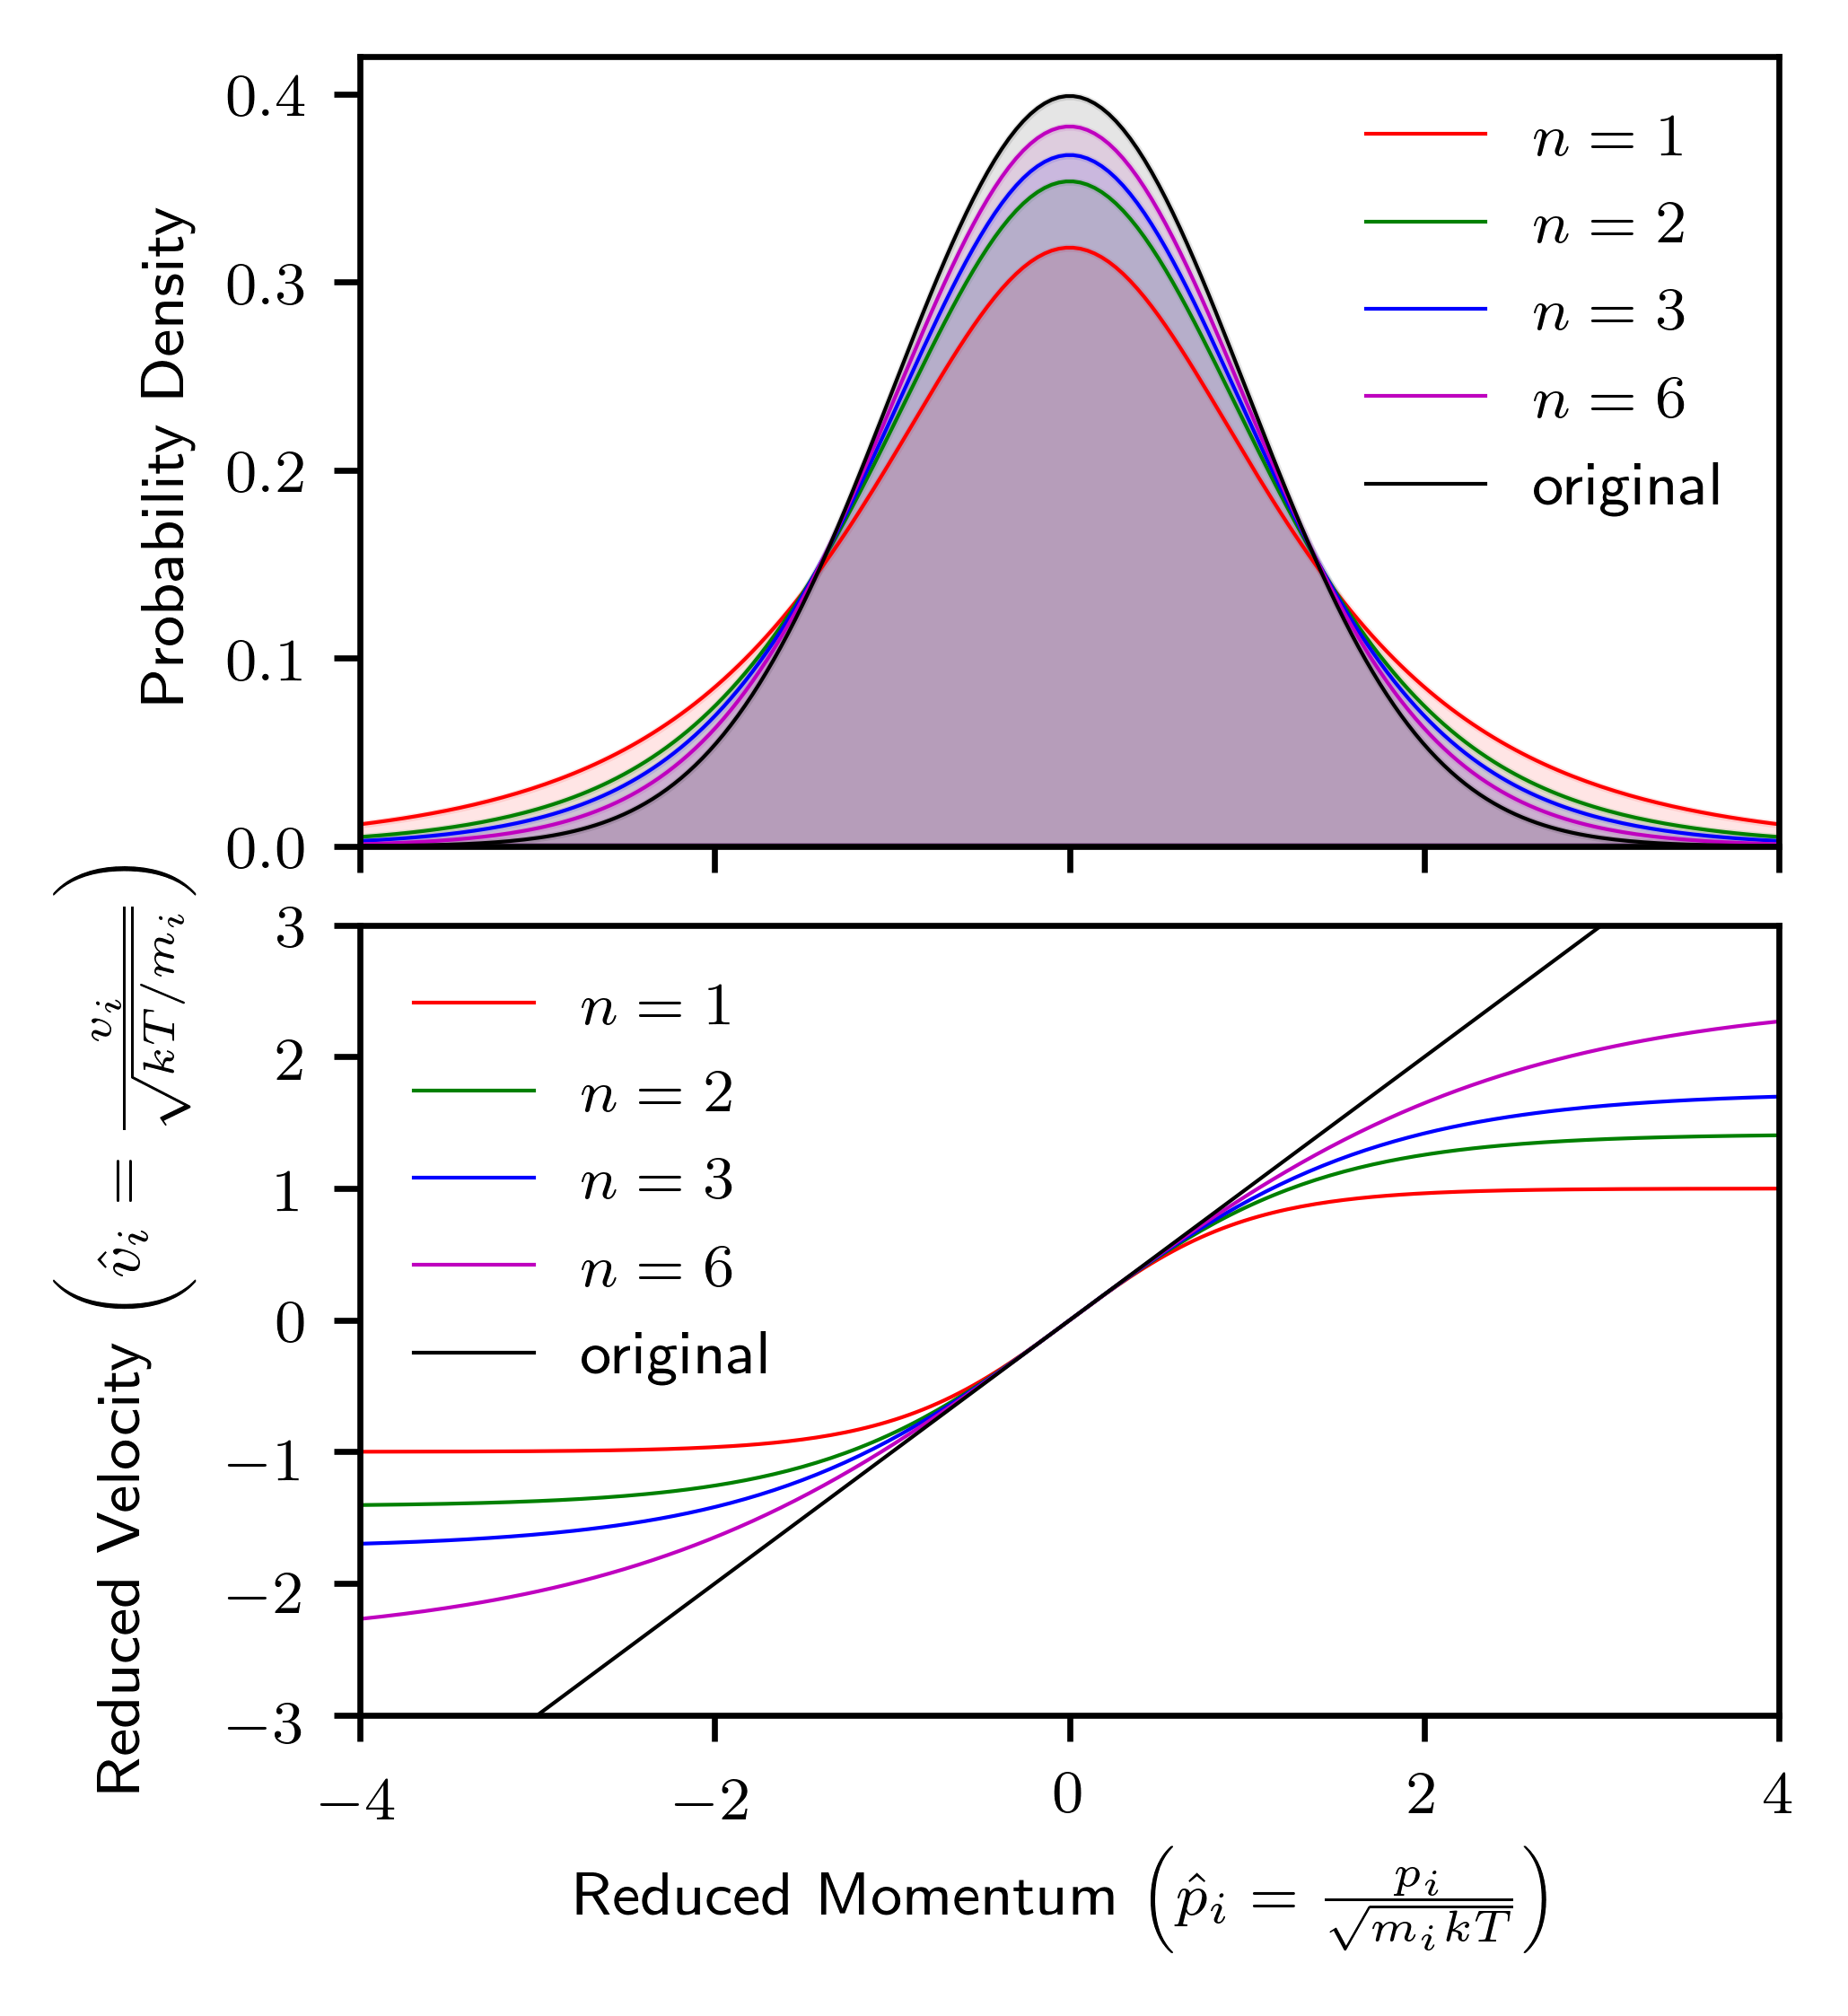
\includegraphics{momentum_functions}
	\caption{Alternative functions for expressing the momentum dependency of the Hamiltonian.}
	\label{fig:hamiltonian momentum dependency}
\end{figure}

The modified Hamiltonian shares important properties with the original one, such as being invariant to momentum sign flips, for instance.
Also, $\mathcal{H}_n$ goes to infinity when $p_i \to \pm \infty$, which is sufficient \cite{Uline_2008} for the validity of Tolman's generalized equipartition theorem,
\begin{equation}
\label{eq:generalized equipartition}
\left\langle v_i p_j \right\rangle = \delta_{ij} k T,
\end{equation}
where $\delta_{ij}$ it the Kronecker delta and $v_i$ is the velocity of degree of freedom $i$, given by 
\begin{equation}
\label{eq:velocity definition}
v_i = \diff{p_i}{{\mathcal H}_n} = \sqrt{\frac{n k T}{m_i}} \tanh\left(\frac{p_i}{\sqrt{n m_i k T}}\right).
\end{equation}

A graphics showing how velocity changes with momentum is presented in Fig.~\ref{fig:hamiltonian momentum dependency}(b).
Note that the new Hamiltonian make $v_i$ hit a plateau when $p_i$ gets too large.
This is different from the standard behavior, in which $v_i$ would keep increasing indefinitely.
In fact, such feature is what provides the modified Hamiltonian with the improved resistance to resonance when employed in multiple time-scale simulations.
In a simulation with the standard Hamiltonian, a large displacement takes place if the absolute value of some momentum increases excessively due to the action of a massive force, thus causing numerical instability.
With the new Hamiltonian, however, displacements with magnitudes above a certain value will never occur.

It is interesting to observe the distribution of velocities, whose PDF is derived in Appendix \ref{sec:momentum and velocity distributions} and depicted in Fig.~\ref{fig:hamiltonian momentum dependency}(b) for multiple $n$ values.
It is given by
\begin{equation*}
\label{eq:velocity distribution}
\varrho_n(v_i) =
\begin{cases}
\frac{\Gamma\left(\frac{n+1}{2}\right)}{\Gamma\left(\frac{n}{2}\right) \sqrt{\frac{n \pi k T}{m_i}}} \left(1-\frac{m_i v_i^2}{n k T}\right)^{\frac{n-2}{2}} & \mathrm{if} \; v_i^2 \leq \frac{n k T}{m_i} \\
0 & \mathrm{otherwise}
\end{cases}.
\end{equation*}

\begin{figure}
	\centering
	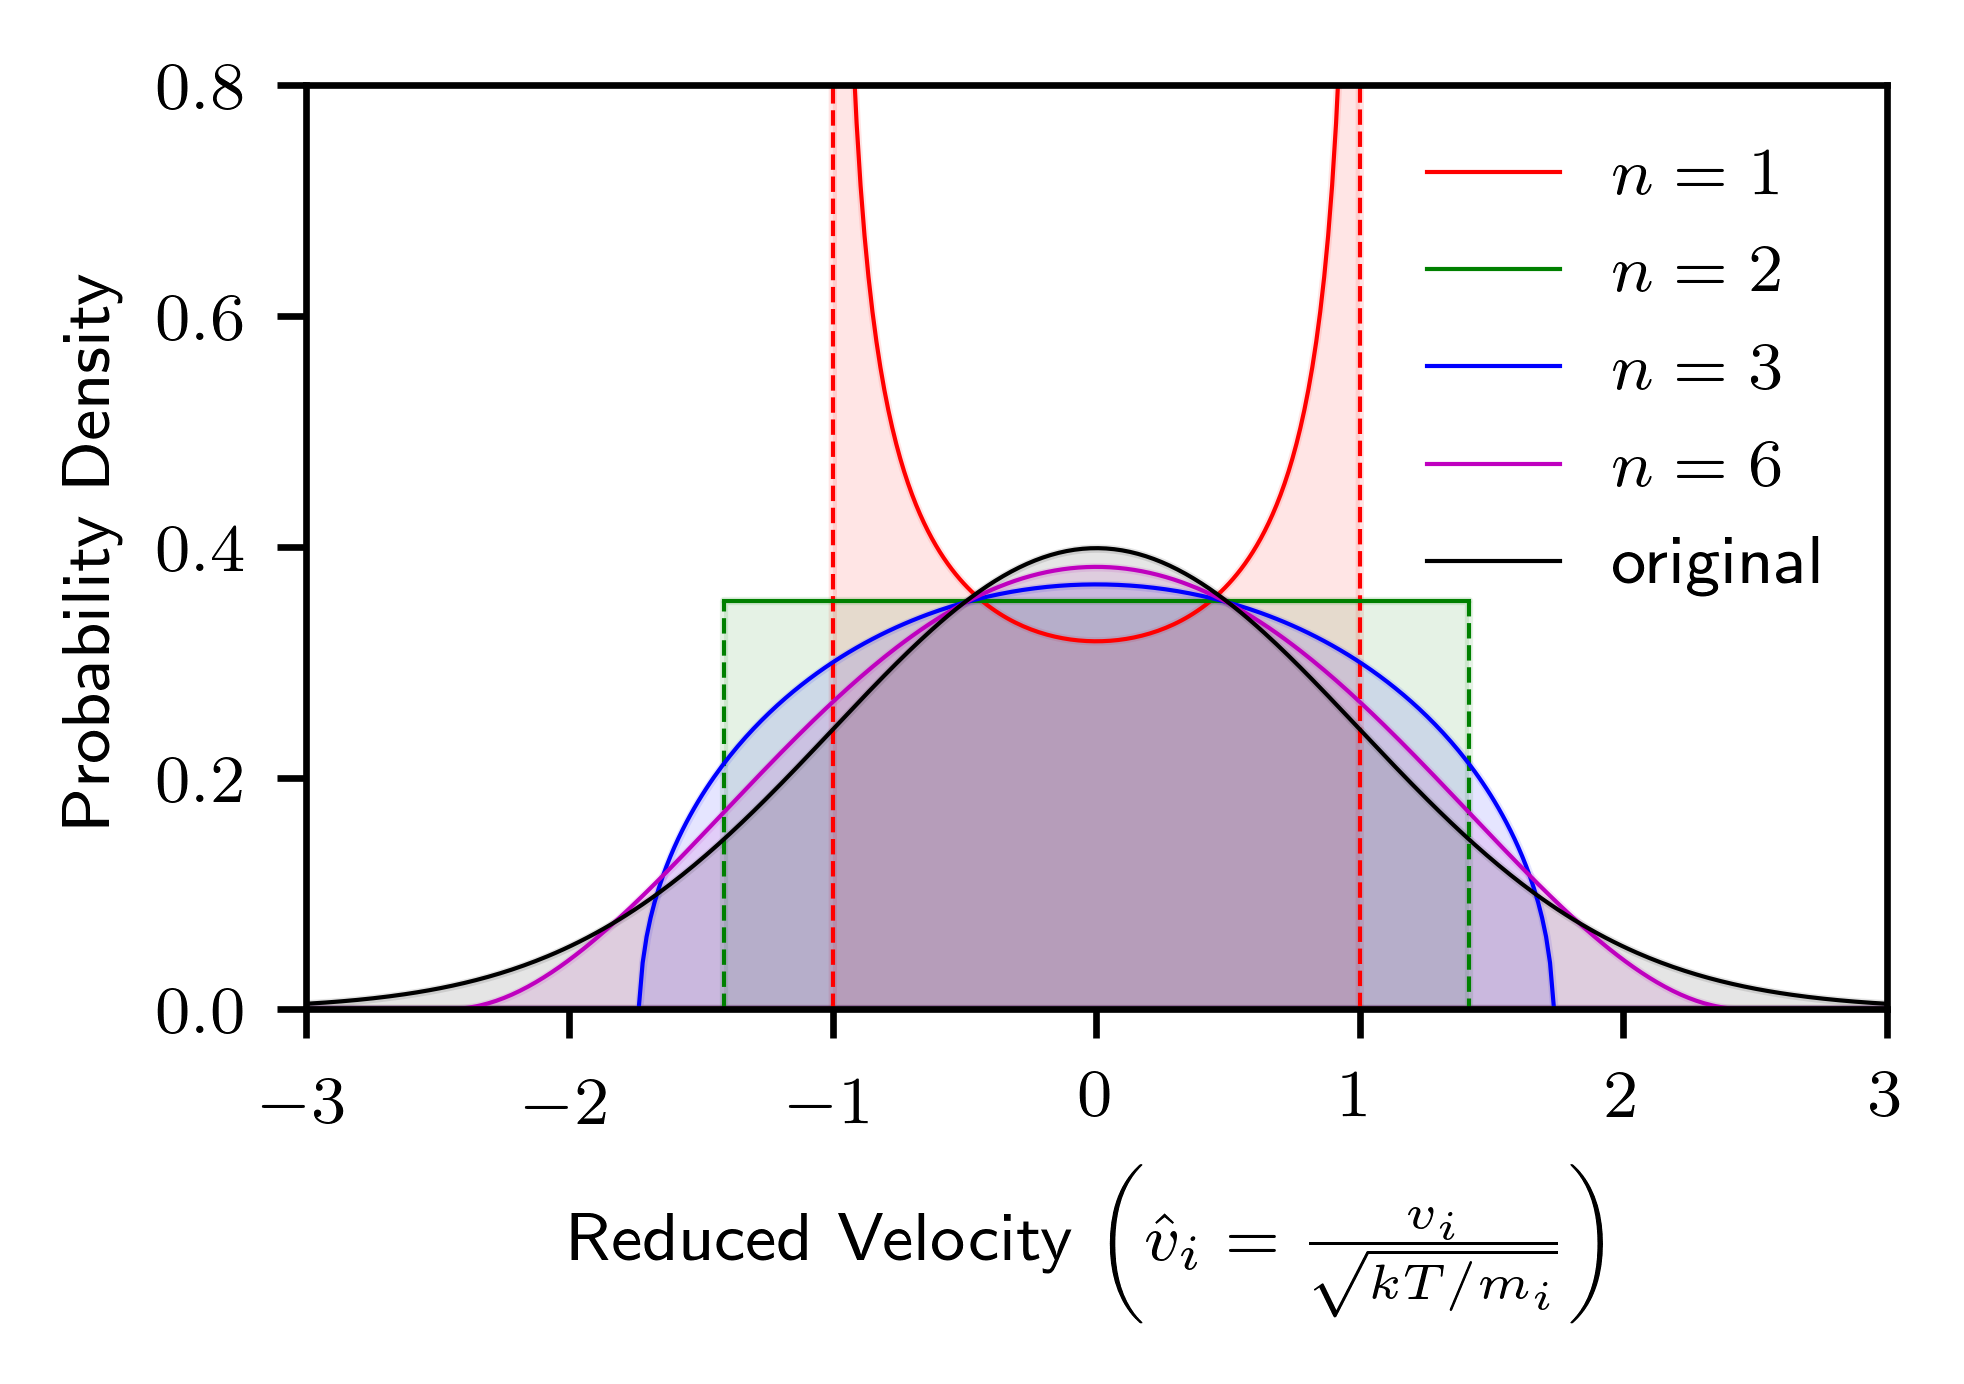
\includegraphics{velocity_distributions}
	\caption{Alternative functions for expressing the momentum dependency of the Hamiltonian.}
	\label{fig:individual momentum distributions}
\end{figure}

This function is akin to using Student's t-distribution with a negative degree-of-freedom parameter.
As seen in Fig.~\ref{fig:hamiltonian momentum dependency}(b), it exhibits an odd behavior for $n \leq 3$, but this seems to have little practical implications, as will be shown in Sec.~\ref{sec:velocity distributions results}.
One important aspect, which will be essential in the forthcoming discussion about thermostat algorithms, is the relation between temperature and the mean-square velocity of each degree of freedom.
From the developments in Appendix~\ref{sec:momentum and velocity distributions}, it follows that
\begin{equation}
\label{eq:mean-square velocity}
\left\langle v_i^2 \right\rangle = \frac{n}{n+1} \frac{kT}{m_i},
\end{equation}
which converges to the standard form when $n \to \infty$, as expected.

\subsection{Massive Nos\'{e}-Hoover Chain Thermostatting}
\label{sec:massive NHC thermostatting}

In our first effort to derive equations of motion for NVT dynamics with the new Hamiltonian, we employ a massive-thermostatting version of the Nos\'{e}-Hoover chain (NHC) method \cite{Martyna_1992}.
This starts by defining an extended phase space with $m \times N_f$ extra coordinates $\vt \eta$ and their conjugate velocities $\vt v_\eta$, where $m$ is the number of thermostats in the chain attached to each degree of freedom.
It is possible to apply the method exactly as it is usually presented, with the equations of motion written in terms of particle momenta.
For this, we define a quantity $H_n$ to be conserved in place of the Hamiltonian $\mathcal{H}_n$, which is
\begin{equation*}
%H_n = {\mathcal H}_n + \sum_{j=1}^m \sum_{i=1}^{N_f} \left(k T \eta_{j, i} + \frac{p_{\eta_{j, i}}^2}{2 Q} \right),
H_n = {\mathcal H}_n + \sum_{i=1}^{N_f} \sum_{j=1}^m \left(k T \eta_{j, i} + \frac{Q v_{\eta_{j, i}}^2}{2} \right),
\end{equation*}
where $Q$ is an inertial parameter.
Equations of motion devised to preserve $H_n$ can be written in the general form \cite{Sergi_2001}
\begin{equation*}
\dot{\vt x} = {\mt B} \nabla_{\vt x}{H_n},
\end{equation*}
where $\mt B$ is a skew-symmetric, matrix-valued function of the dynamic variables in $\vt x$.
%The reason is that, by virtue of the chain rule, the time derivative of a scalar function $f(\vt x)$ is given by $\dot f = \tr{\dot{\vt x}}\diff{\vt x}{f} = \tr{(\diff{\vt x}{H_n})}\tr{\mt B}\diff{\vt x}{f}$. 
%If $f = H_n$, then we have a quadratic form, which is identically null if $\tr{\mt B} = -{\mt B}$.
%The particular form of the NHC system of equations is
%\begin{subequations}
%	\label{eq:general NHC}
%	\begin{align}
%	&\dot{r}_i = \diff{p_i}{H_n} \\
%	&\dot{p}_i = -\diff{r_i}{H_n} -p_i \diff{p_{\eta_{1,i}}}{H_n} \label{eq:general NHC p} \\
%	&\dot{\eta}_{j, i} = \diff{p_{\eta_{j, i}}}{H_n} \\
%	&\dot{p}_{\eta_{1, i}} = p_i \diff{p_i}{H_n} - \diff{\eta_{1, i}}{H_n} - p_{\eta_{1, i}} \diff{p_{\eta_{2, i}}}{H_n} \label{eq:general NHC p_eta_1} \\
%	&\dot{p}_{\eta_{j, i}} = p_{\eta_{j-1, i}} \diff{p_{\eta_{j-1, i}}}{H_n} - \diff{\eta_{j, i}}{H_n} - p_{\eta_{j, i}} \diff{p_{\eta_{j+1, i}}}{H_n} \\
%	&\dot{p}_{\eta_{m, i}} = p_{\eta_{m-1, i}} \diff{p_{\eta_{m-1, i}}}{H_n} - \diff{\eta_{m, i}}{H_n}
%	\end{align}
%\end{subequations}
After all derivatives of $H_n$ have been evaluated, the particular form of the massive-NHC equations of motion is
%\begin{align*}
%&\dot{r}_i = v_i \\
%&\dot{p}_i = F_i - \frac{p_{\eta_{1,i}}}{Q} p_i \\
%&\dot{\eta}_{j,i} = \frac{p_{\eta_{j,i}}}{Q} \\
%&\dot{p}_{\eta_{1, i}} = m_i v_i p_i - kT - \frac{p_{\eta_{2,i}}}{Q} p_{\eta_{1, i}} \\
%&\dot{p}_{\eta_{j, i}} = \frac{p_{\eta_{j-1, i}}^2}{Q} - kT - \frac{p_{\eta_{j+1, i}}}{Q} p_{\eta_{j, i}} \\
%&\dot{p}_{\eta_{m, i}} = \frac{p_{\eta_{m-1, i}}}{Q} p_{\eta_{m-1, i}} - kT
%\end{align*}
\begin{subequations}
	\label{eq:NHC equations}
	\begin{align}
	&\dot{r}_i = v_i, \\
	&\dot{p}_i = F_i - v_{\eta_{1,i}} p_i, \label{eq:NHC equations p} \\
	&\dot{\eta}_{j,i} = v_{\eta_{j,i}}, \\
	&\dot{v}_{\eta_{1, i}} = \frac{v_i p_i - kT}{Q} - v_{\eta_{2, i}} v_{\eta_{1, i}}, \quad \mathrm{and}  \label{eq:NHC equations v_eta_1} \\
	&\dot{v}_{\eta_{j, i}} = \frac{Q v_{\eta_{j-1, i}}^2 - kT}{Q} - v_{\eta_{j+1, i}} v_{\eta_{j, i}} \quad \mathrm{for} \quad j > 1.
	\end{align}
\end{subequations}

In these equations, $v_i$ is a function of $p_i$ as in Eq.~\eqref{eq:velocity definition},
$F_i = -\diff{r_i}{U}$ is the force acting on degree of freedom $i$,
%$G_{j, i} = Q v_{\eta_{j-1, i}}^2 - kT$ is the force that drives the corresponding thermostat,
and $v_{\eta_{m+1, i}} = 0$ by definition.
The velocity $v_i$ depends on $p_i$ via Eq.~\eqref{eq:velocity definition}, which keeps it from assuming any value beyond $\pm \sqrt{{n kT}/{m_i}}$.
The $\eta_{j, i}$ quantities are driven variables and, therefore, it is not actually necessary to integrate them, unless one wishes to validate a numerical method by checking the conservation of $H_n$.
From a theoretical standpoint, however, their presence is crucial for demonstrating that the original phase space is correctly sampled in accordance with $e^{-\frac{\mathcal{H}_n(\vt r, \vt p)}{kT}}$.

A non-Hamiltonian flow in extended space preserves a measure identified by a metric determinant $\sqrt{g} = e^{-w(\vt x)}$, where $w(\vt x)$ satisfies the equation \cite{Tuckerman_1999, Tuckerman_2001}
\begin{equation}
\label{eq:extended space compressibility}
\dot{w} = \nabla_{\vt x} \cdot \dot{\vt x},
\end{equation}
where the divergence represents the extended space compressibility.
In the specific case of Eq.~\eqref{eq:NHC equations},
\begin{equation}
\dot{w} = -\sum_{i=1}^{N_f} \sum_{j=1}^m v_{\eta_{j,i}} = -\frac{d\eta_{\rm sum}}{dt},
\end{equation}
where $\eta_\mathrm{sum} = \sum_{i=1}^{N_f} \sum_{j=1}^m \eta_{j,i}$.
Therefore, $\sqrt{g} = e^{\eta_\mathrm{sum}}$.
Here we note that all $\eta$'s are driven variables and no combinations thereof, other than $\eta_\mathrm{sum}$, is of primary importance \citenum{Tuckerman_2001}.
Thus, following the guidelines of Ref.~\citenum{Tuckerman_2001}, only $\eta_\mathrm{sum}$ is considered in our phase space analysis.
If $H_n$ is the only conserved quantity, then the partition function of the resulting ensemble can be expressed as
\begin{multline}
\label{eq:NHC defined partition function}
\Omega = C_1 \int \delta\left(\mathcal{H}_n + kT\eta_{\rm sum} + K_\eta - H_n^0\right) \\
\times e^{\eta_{\rm sum}}  d{\vt r} d{\vt p} d{\vt v}_\eta d\eta_{\rm sum},
\end{multline}
where $H_n^0$ is a constant that depends on system specification,
$K_\eta$ is the total kinetic energy of the thermostat chain,
and $C_1$ is the proper statistical-mechanical prefactor.
Integrating over $\eta_\mathrm{sum}$ yields
\begin{equation}
\label{eq:NHC partition function}
\Omega = \frac{C_1 e^{-\frac{H_n^0}{kT}}}{kT} \int e^{-\frac{K_\eta}{kT}} d{\vt v}_\eta \int e^{-\frac{\mathcal{H}_n}{kT}}  d{\vt r} d{\vt p} ,
\end{equation}
which is clearly canonical in the original phase space.

\subsection{Modified Nos\'{e}-Hoover Chain and Equivalence to the Isokinetic-NHC Method}

%Because
%\begin{equation}
%\delta\left(g(z)\right) = \frac{\delta(z - z_0)}{|g^\prime(x_0)|},
%\end{equation}
%where $z_0$ is a root of $g(z)$, we can rewrite Eq.~\eqref{eq:NHC defined partition function} as
%\begin{equation}
%\label{eq:NHC partition function}
%\Omega = \int d\vt x \frac{\delta\left(\eta_{\rm sum} + \frac{\mathcal{H}_n + K_\eta - C}{kT}\right)}{kT}e^{\eta_{\rm sum}},
%\end{equation}

In Eq.~\eqref{eq:NHC equations}, thermostatting is enacted by the generalized equipartition theorem, expressed as in Eq.~\eqref{eq:generalized equipartition}.
Nevertheless, in order to establish the equivalence between our proposition and the isokinetic approach, it is necessary to do some small modifications in the NHC equations.
This is so because, as we are going to demonstrate, the principle behind thermostatting in the isokinetic method is Eq.~\eqref{eq:mean-square velocity}, rather than Eq.~\eqref{eq:generalized equipartition}.
First, we substitute $m_i v_i$ for the factor $p_i$ in both Eqs.~\eqref{eq:NHC equations v_eta_1} and \eqref{eq:NHC equations p}.
Next, in order to comply with Eq.~\eqref{eq:mean-square velocity}, we multiply $\frac{n+1}{n}$ by $m_i v_i^2$ in the resulting thermostat equation.
Note that these changes do not keep the dynamics from approaching the original NHC algorithm with standard Hamiltonian \cite{Martyna_1992} when $n \to \infty$.
For a finite $n$, however, the skew-symmetric structure of matrix $\mt B$ is broken, meaning that $H_n$ will no longer be conserved.
The extended-space compressibility changes as well, but our analysis will show that the stationary distribution correctly projects into the original phase space as proportional to $e^{-\frac{\mathcal{H}_n(\vt r, \vt p)}{kT}}$.
This requires introducing a new driven variable for every degree of freedom $i$, in substitution to the set $\{\eta_{j, i} \mid {j\in[1,n]}\}$.
Once again, one does not need to integrate these driven variables in practice, but they are key for proving the method's correctness.
The new equations of motion are
\begin{subequations}
	\label{eq:isokinetic NHC equations}
	\begin{align}
	&\dot{r}_i = v_i, \\
	&\dot{p}_i = F_i - v_{\eta_{1,i}} m_i v_i, \label{eq:isokinetic NHC equations p} \\
	&\dot{\theta}_i = -\left(F_i - v_{\eta_{1,i}} m_i v_i\right)\frac{v_i \theta_i}{k T}, \label{eq:isokinetic NHC equations theta} \\
	&\dot{v}_{\eta_{1, i}} = \frac{\frac{n+1}{n} m_i v_i^2 - kT}{Q} - v_{\eta_{2, i}} v_{\eta_{1, i}}, \quad \mathrm{and} \label{eq:isokinetic NHC equations v_eta_1} \\
	&\dot{v}_{\eta_{j, i}} = \frac{Q v_{\eta_{j-1, i}}^2 - kT}{Q} - v_{\eta_{j+1, i}} v_{\eta_{j, i}} \quad \mathrm{for} \quad j > 1. \label{eq:adapted NHC equations v_eta_j}
	\end{align}
\end{subequations}

Note that $\theta_i$ can never switch sign because its own rate of change vanishes when its value approaches zero.
Here we will consider that $\theta_i$ is always positive, by convention.
The equation above have two very important properties.
First, the metric determinant they imply is given by
\begin{equation}
\label{eq:isokinetic NHC metric determinant}
\sqrt{g} = e^{-\frac{U + K_\eta}{kT}}.
\end{equation}

Second, a new conservation law emerges for every degree of freedom $i$, with a preserved quantity given by
\begin{equation}
\label{eq:isokinetic NHC conserved quantity}
\Phi_i = \theta_i \cosh^n\left(\frac{p_i}{\sqrt{n m_i k T}}\right).
\end{equation}

Mathematical proofs of both properties are provided in Appendix~\ref{sec:adapted NHC proofs}.
Even though each $\theta_i$ is a driven variable, its presence in this conservation law makes it of primary importance \cite{Tuckerman_2001} and requires its inclusion in the phase space analysis.
As a consequence, the partition function of the extended-space ensemble defined by Eq.~\eqref{eq:isokinetic NHC equations} is
\begin{multline*}
\label{eq:isokinetic NHC defined partition function}
\Omega = C_2 \int \prod_{i=1}^{N_f}\delta\left(\theta_i \cosh^n\left(\tfrac{p_i}{\sqrt{n m_i k T}}\right) - \Phi_i^0\right) \\
\times  e^{-\frac{U + K_\eta}{kT}} d{\vt r} d{\vt p} d{\vt v}_\eta d{\vt \theta}.
\end{multline*}

Integration over all $\theta$'s then makes
\begin{equation*}
\label{eq:isokinetic NHC partition function}
\Omega = C_2 \int e^{-\frac{K_\eta}{kT}} d{\vt v}_\eta \int \frac{e^{-\frac{U}{kT}}}{\prod_{i=1}^{N_f} \cosh^n\left(\tfrac{p_i}{\sqrt{n m_i k T}}\right)} d{\vt r} d{\vt p}.
\end{equation*}

Due to the definition of $\mathcal{H}_n$ in Eq.~\eqref{eq:modified hamiltonian}, it is straightforward to conclude that the equation above and Eq.~\eqref{eq:NHC partition function} are equivalent.
Therefore, numerically integrating either the standard or the modified NHC equations will provide samples of the same ensemble, at least in the limit of small time steps.
In practice, only small changes are required in well-established NHC integration methods based on operator splitting \cite{Martyna_1996, Tuckerman_2010}.
%The only difference that deserves special attention concerns the effects of operators $e^{-\timestep v_{\eta_{1,i}} p_i \diff{p_i}{}}$ and $e^{-\timestep v_{\eta_{1,i}} v_i \diff{p_i}{}}$, respectively present in the solutions of Eqs.~\eqref{eq:NHC equations} and \eqref{eq:isokinetic NHC equations}.
While the former yields a simple scaling $p_i(t+\delta t) = p_i(t) e^{-v_{\eta_{1,i}} \delta t}$, the latter can be obtained by solving
\begin{equation}
\frac{d \hat{p}_i}{d t} = - v_{\eta_{1,i}} \sqrt{n} \tanh\left(\frac{\hat{p}_i}{\sqrt{n}}\right),
\end{equation}
where $\hat{p}_i = \frac{p_i}{\sqrt{m_i kT}}$ is a reduced momentum and $v_{\eta_{1,i}}$ is considered as a constant.
Since $\cosh x dx = d \sinh x$ and $\cosh x \tanh x = \sinh x$, the solution turns out to be a scaling of $\sinh\left({\hat{p}_i}/{\sqrt{n}}\right)$.
Therefore,
\begin{equation*}
\hat{p}_i(t+\delta t) = \sqrt{n} \arcsinh\left[\sinh \left(\frac{\hat{p}_i(t)}{\sqrt{n}}\right) e^{-v_{\eta_{1,i}} \delta t}\right].
\end{equation*}

It is also possible to express the solution above in terms of velocities, which can be simplified by means of hyperbolic function identities.
The final expression is
\begin{equation}
v_i(t+\delta t) = \frac{v_i(t) e^{-v_{\eta_{1,i}} \delta t}}{\sqrt{\frac{n kT}{m_i} - v_{i}^2(t) + v_i^2(t) e^{-2 v_{\eta_{1,i}} \delta t}}},
\end{equation}
which can be interpreted as a velocity scaling followed by renormalization, which in turn guarantees that the final result will lie in the allowable range.
Because Eq.~\eqref{eq:isokinetic NHC equations p} is the only one in the corresponding system which directly involves the momentum $p_i$, using the equation above in the numerical integration eliminates the need to compute and store $\vt p$ altogether.

Finally, we demonstrate that Eq.~\eqref{eq:isokinetic NHC equations} results in the same projected dynamics as the Isokinetic-NHC method of \citeauthor{Minary_2004} \cite{Minary_2004}.
We start by actually eliminating $p_i$ from the system by way of its relation with $v_i$.
In order to apply the chain rule $\dot{v}_i = \diff{p_i}{v_i} \dot{p}_i$, we deduce from Eq.~\eqref{eq:velocity definition} that
\begin{equation}
\label{eq:velocity derivative wrt momentum}
\frac{d v_i}{d p_i} = \frac{1}{m_i} \left(1 - \frac{m_i v_i^2}{n k T}\right).
\end{equation}

Then, application to Eq.~\eqref{eq:isokinetic NHC equations p} yields
\begin{equation}
\label{eq:v-based NHC equation}
\dot{v}_i = \frac{F_i}{m_i} - \frac{F_i v_i + v_{\eta_{1,i}} (n k T - m_i v_i^2)}{n k T} v_i.
\end{equation}

The next step is to replace $\theta_i$ by a new driven variable defined as $u_i = \sqrt[n]{\theta_i}$.
As differentiation of $u_i$ with respect to time yields $\dot{u}_i = \frac{\dot{\theta}_i}{n \theta_i} u_i$,
we can substitute $\dot{\theta}$ from Eq.~\eqref{eq:isokinetic NHC equations theta} to obtain
\begin{equation}
\label{eq:u equation of motion}
\dot{u}_i = -\frac{F_i v_i - v_{\eta_{1,i}} m_i v_i^2}{n kT} u_i.
\end{equation}

By noting the similarities between Eqs.~\eqref{eq:v-based NHC equation} and \eqref{eq:u equation of motion}, we rewrite them as
\begin{subequations}
\label{eq:original isokinetic equations}
\begin{align}
&\dot{v}_i = \frac{F_i}{m_i} - \lambda_i v_i \quad \mathrm{and} \\
&\dot{u}_i = -(\lambda_i - v_{\eta_{1,i}}) u_i,
\end{align}
\end{subequations}
respectively, where $\lambda_i = \frac{F_i v_i + v_{\eta_{1,i}} (n k T - m_i v_i^2)}{n k T}$.
%\begin{equation}
%\label{eq:lambda definition}
%\lambda_i = \frac{F_i v_i + v_{\eta_{1,i}} (n k T - m_i v_i^2)}{n k T}.
%\end{equation}
%
These turn out to be the same equations of the isokinetic method of Ref.~\citenum{Minary_2004}.
If an initial value is assigned to each $u_i$ so as to satisfy
\begin{equation}
\label{eq:isokinetic statement}
m_i v_i^2 + \alpha u_i^2 = n kT,
\end{equation}
where $\alpha$ is an arbitrary parameter, then this equality will hold at all times.
This can be easily seen if we depart from Eq.~\eqref{eq:original isokinetic equations} to obtain
\begin{equation*}
m_i v_i \dot{v}_i + \alpha u_i \dot{u}_i = (v_{\eta_{1,i}} - \lambda_i)(m_i v_i^2 + \alpha u_i^2 - n k T),
\end{equation*}
which is twice the time-derivative of $m_i v_i^2 + \alpha u_i^2$.
Eq.~\eqref{eq:isokinetic statement} is an isokinetic statement involving $v_i$ and $u_i$.
We do not name it a constraint here, given the fact that $u_i$ is not treated as a true dynamic variable.
In the original Isokinetic NHC method \cite{Minary_2004}, however, it was used as a constraint in the derivation of the equations of motion, with $\lambda_i$ being a Lagrange multiplier to be determined afterwards.
In fact, instead of defining a single variable $u_i$ per degree of freedom, $n$ variables $u_{j, i}$ were introduced in such a way that $\frac{n}{n+1} Q_u \sum_{j=1}^n u_{j, i}^2 = \alpha u_i^2$, where $Q_u$ is an inertial parameter.
In this case, the isokinetic equation becomes
\begin{equation}
m_i v_i^2 + \frac{n}{n+1} Q_u \sum_{j=1}^n u_{j, i}^2 = n kT.
\end{equation}

Finally, if we use this equation to displace $m_i v_i^2$ from Eq.~\eqref{eq:isokinetic NHC equations v_eta_1}, we end up with a convenient form
\begin{equation}
\dot{v}_{\eta_{1, i}} = \frac{nkT - Q_u \sum_{j=1}^n u_{j, i}^2}{Q} - v_{\eta_{2, i}} v_{\eta_{1, i}}.
\end{equation}

This equation represents a single Nos\'{e}-Hoover chain attached to the $n$ variables $u_{j, i}$ altogether.
In the isokinetic method \cite{Minary_2004}, however, a massive thermostatting strategy was also employed at this level, meaning that an independent thermostat chain was attached to each $u_{j, i}$.
This might be overkill in most practical circumstances, and has the key drawback of turning the $u_{j, i}$ variables into actual dynamic (i.e. non-driven) ones.

\subsection{Massive Nos\'{e}-Hoover-Langevin Thermostat and Equivalence to the SIN(R) Method}

Once we have established the equivalence between ....

\subsection{Langevin Dynamics with Modified Hamiltonian: A New Method for Controlling Resonance in Molecular Dynamics}

Using a modified Hamiltonian instead of isokinetic constraints makes it straightforward to rely on Langevin dynamics as a way to sample configurations in accordance with the Gibbs-Boltzmann statistics.
By following \citeauthor{Stoltz_2018} \cite{Stoltz_2018}, who considered the general case in which the kinetic energy part of a separable Hamiltonian is replaced by another function of momenta, we write down a stochastic differential equation (SDE) system for each degree of freedom $i$ as
\begin{subequations}
	\label{eq:Langevin equations}
	\begin{align}
	&dr_i = v_i dt \quad \mathrm{and} \\
	&dp_i = F_i dt - \gamma m_i v_i dt + \sigma_i dW_i,
	\end{align}
\end{subequations}
with $\sigma_i = \sqrt{2 \gamma m_i kT}$ and $v_i$ is a function of $p_i$ such as defined in Eq.~\eqref{eq:velocity definition}.
The probability density function $\rho(\vt r, \vt p) = {Z}^{-1} e^{-\frac{\mathcal{H}_n(\vt r, \vt p)}{kT}}$ is a stationary distribution of the SDE system above because it satisfies the Fokker-Planck equation \cite{Leimkuhler_2015}
\begin{equation}
\diff{t}{\rho} = -i\!L \rho + \sum_{i=1}^{N_f} \left[ \gamma m_i \diff{p_i}{}(\rho v_i) + \frac{\sigma_i^2}{2} \diff{p_i^2}{^2 \rho} \right],
\end{equation}
where $i\!L$ is the Liouville operator corresponding to the modified Hamiltonian, for which $i\!L \mathcal{H}_n = 0$ \cite{Tuckerman_2010}.
This is so because $\diff{t}{\rho} = 0$ as there is no explicit dependence on time, and $i\!L \rho = -\frac{\rho}{kT}i\!L \mathcal{H}_n = 0$.
In addition, after evaluating the remaining derivatives, we end up with
\begin{equation}
\rho \sum_{i=1}^{N_f} \left[ \left(-\gamma m_i + \frac{\sigma_i^2}{2 kT}\right) \left(\frac{v_i^2}{kT} - \frac{d v_i}{d p_i}\right) \right] = 0,
\end{equation}
which is identically satisfied since $\sigma_i^2 = 2 \gamma m_i kT$.

There are several numerical methods available in the literature for solving the standard Langevin equation, in which $v_i(p_i) = p_i/m_i$.
However, adjustment is required for them to become usable for solving Eq.~\eqref{eq:Langevin equations}.
We select the BAOAB integrator \cite{Leimkuhler_2012, Leimkuhler_2013_2} as our starting point due to its outstanding efficiency in reproducing canonical statistics of configurations.
It consists in applying, at each time step of size $\timestep$, a split propagator defined as
\begin{equation}
e^{\timestep \mathcal{L}_\textsc{BAOAB}} =
e^{\frac{\timestep}{2} \mathcal{L}_B}
e^{\frac{\timestep}{2} \mathcal{L}_A}
e^{\timestep \mathcal{L}_O}
e^{\frac{\timestep}{2} \mathcal{L}_A}
e^{\frac{\timestep}{2} \mathcal{L}_B},
\end{equation}
whose each factor represents the exact solution of a simpler subproblem.
The division can be depicted \cite{Leimkuhler_2015} as
\begin{equation}
\left[\begin{array}{c}
dr_i \\ dp_i
\end{array}\right] =
\underbrace{\left[\begin{array}{c}
v_i dt \\ 0
\end{array}\right]}_\mathrm{A} + 
\underbrace{\left[\begin{array}{c}
0 \\ F_i dt
\end{array}\right]}_\mathrm{B} +
\underbrace{\left[\begin{array}{c}
0 \\ -\gamma m_i v_i dt + \sigma_i dW_i
\end{array}\right]}_\mathrm{O}.
\end{equation}

Hence, the effects of propagators $e^{\delta t \mathcal{L}_A}$ and $e^{\delta t \mathcal{L}_B}$ are a displacement given by $r_i(t+\delta t) = r_i(t) + v_i(t) \delta t$ and an impulse given by $p_i(t+\delta t) = p_i(t) + F_i(t) \delta t$, respectively.
In the traditional case, the remaining propagator, $e^{t \mathcal{L}_O}$, represents an Ornstein-Uhlenbeck (OU) process and, as such, its effect can be evaluated exactly (in the stochastic sense) from a closed-form solution of the linear SDE
\begin{equation}
\label{eq:traditional Langevin}
d\hat{p}_i = - \gamma \hat{p}_i dt + \sqrt{2 \gamma} dW_i,
\end{equation}
which is
\begin{equation}
\label{eq:Ornestein-Uhlenbeck solution}
\hat{p}_i(t+\delta t) = e^{-\gamma \delta t} \hat{p}_i(t) + \sqrt{1 - e^{-2 \gamma \delta t}} \xi_i,
\end{equation}
where $\xi_i$ is an independent, standard normal random variable.
In the present case, however, this propagator represents the joint solution for all $i$ of a non-linear stochastic process given by
\begin{equation}
\label{eq:Langevin equation with new velocity}
d\hat{p}_i = - \gamma \sqrt{n} \tanh\left(\frac{\hat{p}_i}{\sqrt{n}}\right) dt + \sqrt{2 \gamma} dW_i,
\end{equation}
which is not an OU process and has no simple analytical solution.
Some approximation is thus required.
In the present work, we consider and empirically test two approximate solutions, described as follows.

\subsubsection{Non-Linear Extension of the Gr{\o}nbech-Jensen \& Farago Integrator}

The Langevin integrator proposed by \citeauthor{Gronbech-jensen_2013} \cite{Gronbech-jensen_2013} (GJF) has also been observed to show excellent performance at sampling configurations in accordance with the canonical distribution \cite{Jensen_2019, Farago_2019, Finkelstein_2019}.
A little-known fact about this integrator is its incidentally close correspondence with the BAOAB splitting (\citeauthor{Li_2017} \cite{Li_2017}, Appendix B).
In fact, it is possible to derive the GJF method by simply replacing the exact OU solution in the BAOAB scheme by a numerical approximation.
Integrating both sides of Eq.~\eqref{eq:traditional Langevin} yields
\begin{equation*}
\hat{p}_i(t+\delta t) - \hat{p}_i(t) = - \gamma \int_t^{t+\delta t} \hat{p}_i(s) ds + \sqrt{2 \gamma \delta t} \xi_i.
\end{equation*}

Then, by using the trapezoidal rule to evaluate the remaining integral, we obtain
\begin{equation}
\label{eq:GJF approximation}
\hat{p}_i(t+\delta t) \approx a \hat{p}_i(t) + b \sqrt{2 \gamma \delta t} \xi_i,
\end{equation}
where $b = (1 + \tfrac{\gamma \delta t}{2})^{-1}$ and $a = b (1 - \tfrac{\gamma \delta t}{2})$.
Following Ref.~\citenum{Li_2017}, another possible interpretation is that GJF corresponds to using BAOAB with an approximate friction constant given by $\gamma^\ast = -\timestep^{-1} \ln a$.
This explains why GJF reproduces the equilibrium statistics of harmonic oscillators as accurately as BAOAB does \cite{Jensen_2019, Farago_2019, Finkelstein_2019}, since it has long been known that the latter yields a coordinate-momentum covariance matrix that does not depend on the friction constant \cite{Leimkuhler_2013_2}.
It is interesting, though, that in a recent observation of molecular diffusion in the large-friction regime ($\gamma \approx  0.1~\mathrm{fs}^{-1}$) BAOAB seems to deviate from the expected behavior as the time-step size increases, whereas GJF keeps giving the correct results.
Because splitting is itself an approximation, employing an approximate step in place of its exact counterpart might be causing some error compensation.

In view of the good performance of the GJF method, the same trapezoidal-rule procedure can be applied to obtain a solution for Eq.~\eqref{eq:Langevin equation with new velocity}.
In this case, however, as we cannot isolate $p_i(t+\delta)$ from the resulting equation, its value must be computed self-consistently.
For instance, we can use
\begin{equation}
%\hat{p}_i = \hat{p}_i - \frac{\hat{p}_i + \frac{\gamma \timestep}{2} \sqrt{n} \tanh \left(\frac{\hat{p}_i}{\sqrt{n}}\right) - C}{1 + \frac{\gamma \timestep}{2} \left[1 - \tanh^2 \left(\frac{\hat{p}_i}{\sqrt{n}}\right) \right]},
\hat{p}_i = \hat{p}_i - \frac{\hat{p}_i + \frac{\gamma \timestep}{2} \hat{v}_i - C}{1 + \frac{\gamma \timestep}{2} \left(1 - \frac{\hat{v}_i^2}{n} \right)},
\end{equation}
where $\hat{v}_i = \sqrt{n} \tanh\left(\frac{\hat{p}_i}{\sqrt{n}}\right)$ and $C = \hat{p}_i(t) - \frac{\gamma \delta t}{2} \hat{v}_i(t) + \sqrt{2 \gamma \delta t} \xi_i$.
This comes from applying the Newton-Raphson method to a monotonic function of $\hat{p}_i$, which makes it quadratically convergent.
With the same value of $\xi_i$ as in the $C$ constant, either Eq.~\eqref{eq:Ornestein-Uhlenbeck solution} or Eq.~\eqref{eq:GJF approximation} is expected to provide a suitable initial guess.

\subsubsection{Splitting-Based Solution of a Perturbed Ornstein-Uhlenbeck Process}

By defining a perturbation function $\hat{z}_i(\hat{p}_i)$ as
\begin{equation}
z_i = \sqrt{n} \tanh\left(\frac{\hat{p}_i}{\sqrt{n}}\right) - \hat{p}_i,
\end{equation}
we can rewrite Eq.~\eqref{eq:Langevin equation with new velocity} as
\begin{equation}
\label{eq:Langevin equation with perturbed OU process}
d\hat{p}_i = \underbrace{- \gamma \hat{p}_i dt + \sqrt{2 \gamma} dW_i}_{OU} - \gamma \hat{z}_i dt.
\end{equation}

It is clear that $z_i$ is mostly relevant for small values of $n$, but vanishes as $n \to \infty$.
We propose a splitting solution for the equation above in which an exact OU step is surrounded by correction steps, that is,
\begin{equation*}
e^{\timestep \mathcal{L}_O} =
e^{\frac{\timestep}{2} \gamma \hat{\vt p} \cdot \nabla_{\hat{\vt p}}}
e^{-\frac{\timestep}{2} \gamma \hat{\vt v} \cdot \nabla_{\hat{\vt p}}}
e^{\timestep \mathcal{L}_\mathrm{OU}}
e^{-\frac{\timestep}{2} \gamma \hat{\vt v} \cdot \nabla_{\hat{\vt p}}}
e^{\frac{\timestep}{2} \gamma \hat{\vt p} \cdot \nabla_{\hat{\vt p}}}.
\end{equation*}


\citeauthor{Stoltz_2018} \cite{Stoltz_2018} have shown that splitting solutions applied to stochastic equations such as Eq.~\eqref{eq:Langevin equation with new velocity} can converge to a stationary distribution because $|\hat{v}_i - \hat{p}_i|$ 

\cite{Trstanova_2016}

considered the convergence of


we can expect that will converge to a stationary distribution, since $| m_i v_i - p_i |$ is bounded.


\begin{equation}
e^{\frac{\timestep}{2} \mathcal{L}_{Z}} =
e^{\frac{\timestep}{4} \gamma \hat{p}_i \diff{\hat{p}_i}{}}
e^{-\frac{\timestep}{2}  \gamma \hat{v}_i \diff{\hat{p}_i}{}}
e^{\frac{\timestep}{4} \gamma \hat{p}_i \diff{\hat{p}_i}{}}
\end{equation}

\begin{equation*}
e^{\timestep \mathcal{L}_O} =
e^{\frac{\timestep}{2} \gamma \hat{\vt p} \cdot \nabla_{\hat{\vt p}}}
e^{\frac{\timestep}{2} \gamma \hat{\vt v} \cdot \nabla_{\hat{\vt p}}}
e^{\timestep \mathcal{L}_\mathrm{OU}}
e^{\frac{\timestep}{2} \gamma \hat{\vt v} \cdot \nabla_{\hat{\vt p}}}
e^{\frac{\timestep}{2} \gamma \hat{\vt p} \cdot \nabla_{\hat{\vt p}}}
\end{equation*}


By composing the three steps in a single equation, the effect of propagator $e^{\delta t \mathcal{L}_{Z}}$ can be represented by
\begin{equation*}
\hat{p}_i(t+\delta t) = e^{\frac{\gamma \delta t}{2}} \sqrt{n} \arcsinh\left[\sinh\left(\frac{\hat{p}_i(t) e^{\frac{\gamma \delta t}{2}}}{\sqrt{n}}\right) e^{-\gamma \delta t} \right].
\end{equation*}

Unfortunately, linear analysis is not possible.

\section{Results}

\subsection{Numerical Integration of the Modified Stochastic Propagator}

The fact that 

Order-1.5 Strong It\={o}-Taylor Scheme \cite{Kloeden_1992}
\begin{multline}
p_i(t+\delta t) = \hat{p}_i(t) - \hat{v}_i(t) \gamma \delta t + \sqrt{2 \gamma \delta t} \xi_{i,1} - \left(1 - \frac{\hat{v}_i(t)^2}{n}\right) \times \\
\times \left[ \frac{\sqrt{2 \gamma^3 \delta t^3}}{2}\left(\xi_{i,1} + \frac{\xi_{i,2}}{\sqrt{3}}\right) - \frac{n+2}{2 n} \hat{v}_i(t) \gamma^2 \delta t^2 \right],
\end{multline}

\begin{figure}
	\centering
	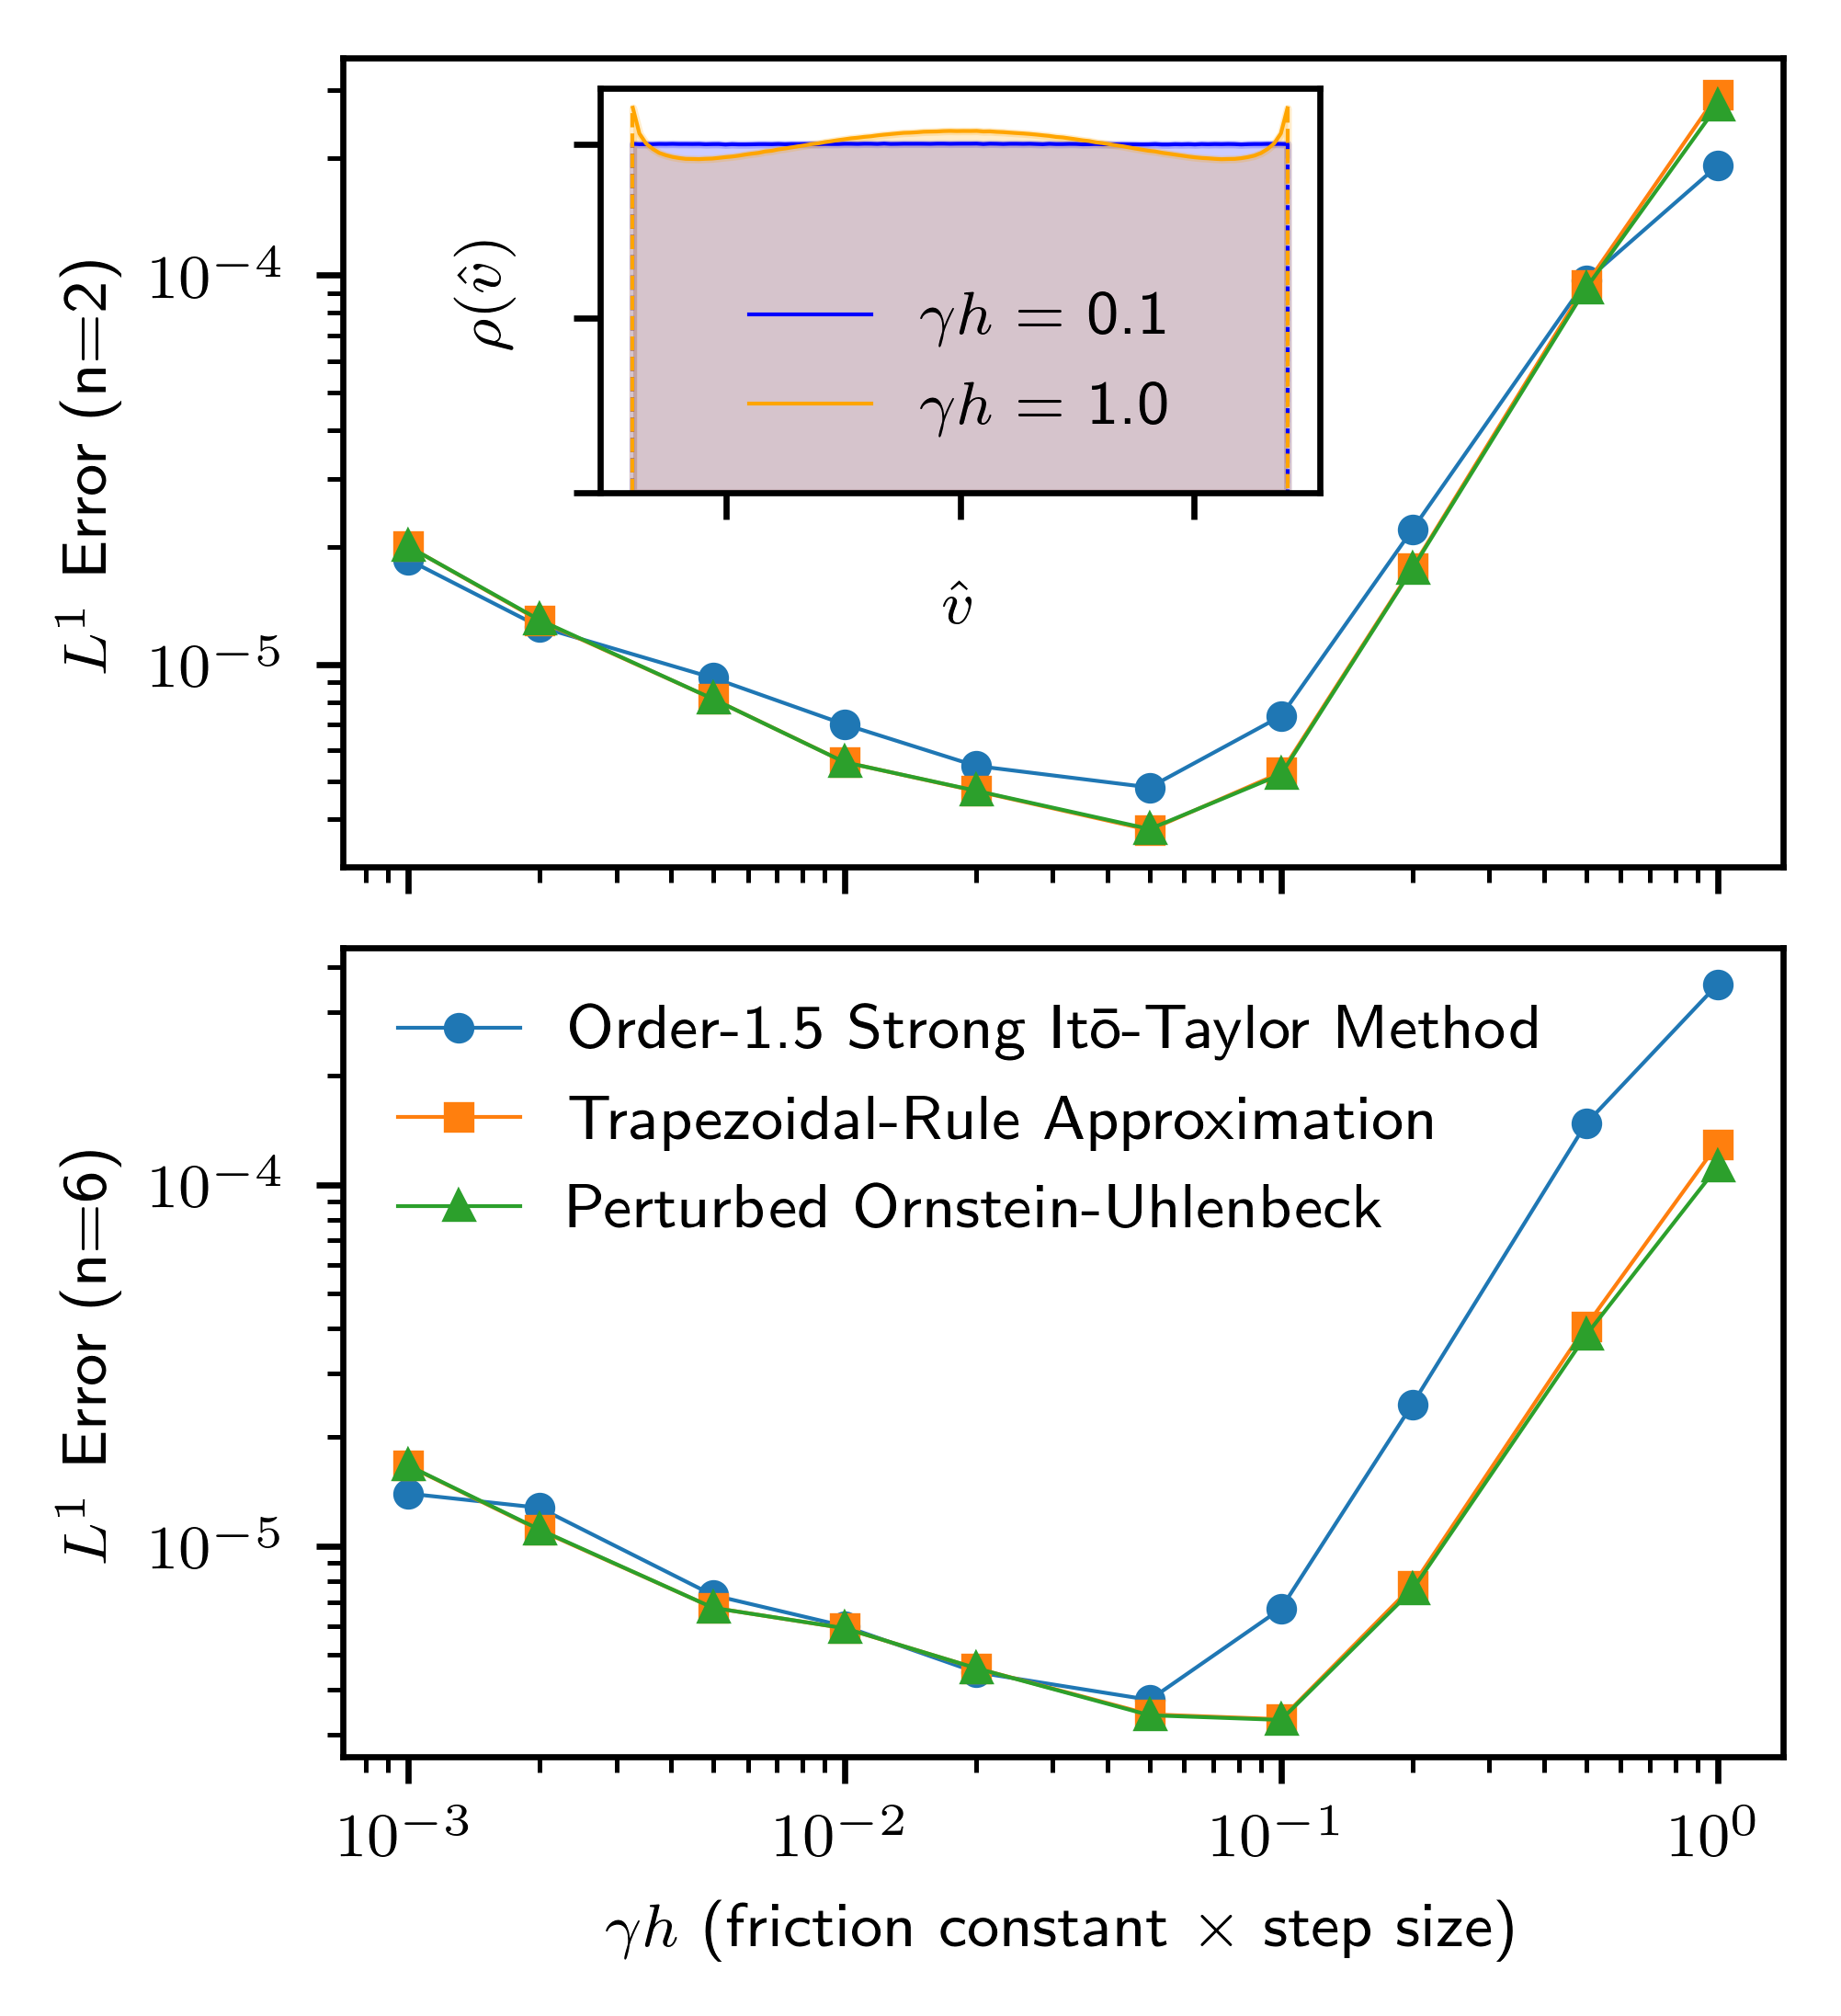
\includegraphics{stochastic_integration}
	\caption{Alternative functions for expressing the momentum dependency of the Hamiltonian.}
	\label{fig:stochastic integration}
\end{figure}



\section{Conclusion}

\appendix

\section{Momentum and Velocity Distributions in a Canonical Ensemble with the Modified Hamiltonian}
\label{sec:momentum and velocity distributions}

In an NVT ensemble corresponding to the Hamiltonian ${\mathcal H}_n$ defined in Eq.~\eqref{eq:modified hamiltonian}, the probability of each momentum $p_i$ is proportional to $e^{-n\ln\cosh(p_i/\sqrt{n m_i kT})}$.
This can be represented as
\begin{equation*}
\rho_n(p_i) = \frac{1}{C_n} \sech^n\left(\frac{p_i}{\sqrt{n m_i k T}}\right),
\end{equation*}
where $C_n$ is a normalization constant.
Because the velocity $v_i$ is a monotonic function of $p_i$, it is straightforward to obtain the velocity probability density $\varrho_n(v_i)$.
Considering that $p_i = f(v_i)$, the relation between the two probability densities is $\varrho_n(v_i) = |f^\prime(v_i)| \rho_n\left(f(v_i)\right)$.
From Eq.~\eqref{eq:velocity definition},
\begin{equation}
\label{eq:momentum as a function of velocity}
f(v_i) = \sqrt{n m_i k T}\arctanh\left(\sqrt{\frac{m_i}{n k T}} v_i\right).
\end{equation}

%Therefore,
%\begin{equation*}
%\varrho_n(v_i) = \frac{m_i}{\left|1-\frac{m_i v_i^2}{n k T}\right|} \frac{1}{C_n} \sech^n\left(\arctanh\left(\sqrt{\frac{m_i}{n k T}} v_i\right)\right).
%\end{equation*}

Next, the identity $\sech(\arctanh(y)) = \sqrt{1-y^2}$ and the fact that $v_i$ is bounded make
\begin{equation*}
\varrho_n(v_i) = \begin{cases}
\frac{m_i}{C_n} \left(1-\frac{m_i v_i^2}{n k T}\right)^{\frac{n}{2} - 1} & \mathrm{if} \; v_i^2 \leq \frac{n k T}{m_i} \\
0 & \mathrm{otherwise}
\end{cases}.
\end{equation*}

Finally, we can use the fact that $\int_{-\infty}^\infty \varrho_n(v_i) dv_i = 1$ so as to determine an expression for the constant $C_n$.
By changing variables from $v_i$ to $z = \frac{v_i}{\sqrt{{n k T}/{m_i}}}$, we obtain
\begin{equation}
\frac{C_n}{\sqrt{n m_i k T}} = \int_{-1}^{1} (1-z^2)^{\frac{n}{2}-1} dz = \frac{\sqrt{\pi} \Gamma\left(\frac{n}{2}\right)}{\Gamma\left(\frac{n+1}{2}\right)},
\end{equation}
where $\Gamma(\cdot)$ is the (complete) gamma function.
The same change of variables can be use to evaluate the central moments of the velocity distribution.
Because is is symmetric, all odd-order moments are null, and the even-order ones can be obtained by solving
\begin{equation}
\langle z^{2m} \rangle = \frac{\Gamma\left(\frac{n+1}{2}\right)}{\sqrt{\pi} \Gamma\left(\frac{n}{2}\right)} \int_{-1}^{1} z^{2m} (1-z^2)^{\frac{n}{2}-1} dz,
\end{equation}
where $m$ is a positive integer number.
Then, we obtain the general formula
\begin{equation}
\langle v_i^{2m} \rangle = \frac{\Gamma\left(\frac{n+1}{2}\right) \Gamma\left(\frac{2m+1}{2}\right)}{\sqrt{\pi}\Gamma\left(\frac{n+2m+1}{2}\right)} \left(\frac{n k T}{m_i}\right)^m.
\end{equation}

\section{Metric Determinant and Conservation Law for the Modified NHC Equations}
\label{sec:adapted NHC proofs}

The first goal of this appendix is to prove the validity of Eq.~\eqref{eq:isokinetic NHC metric determinant}, which expresses the metric determinant implied by the modified NHC equations of motion.
As another way of representing it, we can state that $\sqrt{g} = e^{-w(\vt r, \vt v_\eta)}$, where $w$ satisfies Eq.~\eqref{eq:extended space compressibility} \cite{Tuckerman_1999, Tuckerman_2001}.
As stated in Sec.~\ref{sec:massive NHC thermostatting}, the time derivative of $w$ can be evaluated by chain rule as $\dot{w} = \tr{\dot{\vt x}} \diff{\vt x}{w}$.
Therefore, what we must prove here is that \cite{Ezra_2004}
\begin{equation}
\label{eq:metric determinant proof equality}
\tr{\dot{\vt x}} \diff{\vt x}{w} = \nabla_{\vt x} \cdot \dot{\vt x},
\end{equation}
with $w$ compliant with Eq.~\eqref{eq:isokinetic NHC metric determinant} and $\dot{\vt x}$ given by Eq.~\eqref{eq:isokinetic NHC equations}.
After evaluation of the $w$ gradient, the left-hand side above reads
\begin{equation*}
\tr{\dot{\vt x}} \diff{\vt x}{w} = \frac{1}{kT} \sum_{i=1}^{N_f} \left(\dot{r}_i \diff{r_i}{U} + \sum_{j=1}^n \dot{v}_{\eta_{j,i}} Q v_{\eta_{j,i}} \right).
\end{equation*}

Next, by substituting the corresponding derivatives from Eq.~\eqref{eq:isokinetic NHC equations}, as well as the definition of force, we obtain
\begin{multline*}
\tr{\dot{\vt x}} \diff{\vt x}{w} = \frac{1}{kT} \sum_{i=1}^{N_f} \Bigg[-F_i v_i \\ 
+ \left(\frac{n+1}{n} m_i v_i^2 - kT - Q v_{\eta_{2, i}} v_{\eta_{1, i}}\right) v_{\eta_{1,i}} \\
+ \sum_{j=2}^n \left(Q v_{\eta_{j-1, i}}^2 - kT - Q v_{\eta_{j+1, i}} v_{\eta_{j, i}}\right) v_{\eta_{j,i}} \Bigg].
\end{multline*}

Many of the terms above cancel out, after which the expression can be simplified to
\begin{multline*}
\tr{\dot{\vt x}} \diff{\vt x}{w} = \sum_{i=1}^{N_f} \bigg[- v_{\eta_{1,i}}\left(1 - \frac{m_i v_i^2}{n kT}\right) \\
-\left(F_i - v_{\eta_{1,i}} m_i v_i\right) \frac{v_i}{kT} - \sum_{j=2}^n v_{\eta_{j,i}} \bigg].
\end{multline*}

We now turn the attention to the right-hand side of Eq.~\eqref{eq:metric determinant proof equality}, which evaluates in accordance with Eq.~\eqref{eq:isokinetic NHC equations} to
\begin{multline*}
\nabla_{\vt x} \cdot \dot{\vt x} = \sum_{i=1}^{N_f} \left(\diff{p_i}{\dot{p}_i} + \diff{\theta_i}{\dot{\theta}_i} + \sum_{j=1}^{n-1} \diff{v_{\eta_{j,i}}}{\dot{v}_{\eta_{j,i}}}\right) = \\
= \sum_{i=1}^{N_f} \Bigg[- v_{\eta_{1,i}} m_i \diff{p_i}{v_i} - \left(F_i - v_{\eta_{1,i}} m_i v_i\right) \frac{v_i}{kT} - \sum_{j=2}^n v_{\eta_{j,i}} \Bigg].
\end{multline*}

Hence, after substitution of Eq.~\eqref{eq:velocity derivative wrt momentum}, it becomes evident by comparison that Eq.~\eqref{eq:metric determinant proof equality} holds.

Our second goal is to prove that the property $\Phi_i$, as expressed in Eq.~\eqref{eq:isokinetic NHC conserved quantity}, is an integral of motion (i.e. a conserved quantity) of the modified NHC dynamics.
By applying a logarithm to both sides of Eq.~\eqref{eq:isokinetic NHC conserved quantity} and differentiating the result with respect to time, we get
%Logarithm:
%\begin{equation}
%\ln \Phi_i = \ln \theta_i + n \ln \cosh\left(\frac{p_i}{\sqrt{n m_i k T}}\right).
%\end{equation}
%
%Taking the time derivative:
\begin{equation}
\frac{d \ln \Phi_i}{dt} = \frac{d \ln \theta_i}{dt} + \sqrt{\frac{n}{m_i kT}}  \tanh\left(\frac{p_i}{\sqrt{n m_i k T}}\right) \frac{d p_i}{dt}.
\end{equation}

Then, with the aid of Eq.~\eqref{eq:velocity definition}, we can write
\begin{equation}
\frac{\dot{\Phi}_i}{\Phi_i} = \frac{\dot{\theta}_i}{\theta_i} + \frac{v_i \dot{p}_i}{kT}.
\end{equation}

Finally, substitution of $ \dot{p}_i$ and $\dot{\theta}_i$ from Eqs.~\eqref{eq:isokinetic NHC equations p} and \eqref{eq:isokinetic NHC equations theta} leads to the conclusion that $\dot{\Phi}_i = 0$.

\bibliography{modified_hamiltonian}

\end{document}